\anexo{Coordenadas Homogêneas}
\label{an:coordenadas-homogeneas}

As coordenadas homogêneas foram criadas para solucionar um problema presente na geometria do espaço Euclidiano, onde duas linhas paralelas no mesmo plano nunca poderão se cruzar. Isso só é interessante até o ponto em que precisamos definir o comportamento geometrico no espaço de projeção. Por exemplo na Figura \ref{fig:projecao} os trilhos se aproximam até que convergem no horizonte (um ponto no infinito no espaço Euclidiano) distante do observador \cite{homogenous}.

	\begin{figure}[h!]
		\centering
		\Caption{\label{fig:projecao} A ferrovia fica mais estreita e se cruza no horizonte.}
		\UNIFORfig{}{
			\fbox{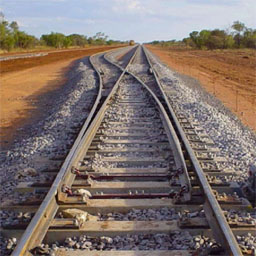
\includegraphics[width=8cm]{figuras/railroad}}
		}{
			\Fonte{\url{http://www.songho.ca/math/homogeneous/homogeneous.html}}
		}
	\end{figure}

Quando um ponto vai para o infinito ele é representado pelas coordenadas ($\infty$, $\infty$) e isso se torna uma informação inexpressiva. As linhas paralelas deveriam se cruzar no espaço de projeção mas não conseguem no espaço Euclidiano. Para resolver esse problema os matemáticos criaram as coordenadas homogêneas \cite{homogenous}.

Coordenadas homogêneas são utilizadas para fazer a representação de coordenadas n-dimensionais utilizando n+1 números. Então para transformar um ponto de duas dimensões no sistema de coordenadas cartesianas (X, Y) basta simplesmente adicionar uma variável, portanto (x, y, w). A correlação matemática entre coordenadas cartesianas e coordenadas homogêneas é exibida abaixo na equação \ref{eq-homogenea}. Utilizando essa lógica fica claro que se um ponto (1, 2), se move em direção ao infinito, se tornando ($\infty$,$\infty$), ele passa a ser representado por (1, 2, 0) em coordenadas homogêneas, conforme a equação \ref{eq-homogenea2} \cite{homogenous}.

\begin{equation} \label{eq-homogenea}
	\begin{aligned}
	X = \cfrac{x}{w} \\
	Y = \cfrac{y}{w} 
	\end{aligned}
\end{equation}

\begin{equation} \label{eq-homogenea2}
	\begin{aligned}
		\left(\cfrac{1}{0}, \cfrac{2}{0}\right) \approx (\infty,\infty)
	\end{aligned}
\end{equation}